\chapter{高效的基于变分推断的高阶依存句法分析}\label{cha:approximate-vi}

本章节提出了一个采用消息传递机制的二阶基于图的和端到端神经网络模型.
这里我们从经验上表明,我们采用的近似方法不仅从准确率上可以与章节~\ref{cha:dep-crf}里提出的二阶基于图的解析器相匹敌,并且其训练和测试的速度都要远远快于二阶CRF解析器.

\section{引言}\label{sec:dep-vi-intro}
基于图的依存句法分析一直以来都是依存句法分析领域的一个比较流行的方法.
在本章节中,我们在章节~\ref{cha:dep-crf}的基础上继续探索基于图的依存句法分析,即给定一个句子,选择将句子分解为多个部分并对他们打分,进而选择分值最高的句法树.

一阶基于图的依存句法分析将一棵完整的句法树分解为多条弧,将每条弧都视为一个独立的部分.
在深度学习时代之前,已经有大量的方法被提出用于一阶依存句法分析\cite{mcdonald-pereira-2006-online,koo-etal-2007-structured,ma-hovy-2017-neural,dozat-etal-2017-biaffine}.

这些方法通常依赖于大量的手工特征的设计,以及结构化学习方法,比如Max Margin、TreeCRF和Matrix Theorem等等,这些方法通常显示建模树的约束,更新参数使得模型尽可能预测出正确的树结构.
得益于深度神经网络的强大上下文建模能力,近期的一些工作通常基于更简单的训练方法.
其中\cite{dozat-etal-2017-biaffine}(Biaffine Parser)提出一个简单的基于头选择目标的解析器,训练时目的是最大化每条弧的头的概率.
他们采用了深度双向LSTM网络作为编码器,并使用了一个双仿射结构的打分器来给依存弧打分.
由于其高效率,并且取得了不逊色于结构化学习方法的结果\cite{zhang-etal-2019-empirical,falenska-kuhn-2019-non},Biaffine Parser是目前最为流行的依存解析器.

与此对应的,

在神经网络时代之前,结构化学习被证明对于
已经有大量的精确推断方法\cite{mcdonald-pereira-2006-online,carreras-2007-experiments,koo-collins-2010-efficient,ma-zhao-2012-fourth}应用于句法分析,旨在找出分值最高的句法树.
近期的一些基于图的工作关注于神经网络方法\cite{chen-manning-2014-fast,kiperwasser-goldberg-2016-simple,dozat-etal-2017-biaffine,ma-hovy-2017-neural}.

后续有工作进一步引入了二阶的推断算法.
\cite{ji-etal-2019-graph}提出利用图神经网络来捕获词的二阶信息,从而进行一阶解析.
\cite{fonseca-martins-2020-revisiting}回顾了可以应用于神经网络模型的高阶解析方法,他们在打分的时候引入了二阶项,然后使用Max Margin方法训练,最大化正确树和其他树的分值边际.
我们在章节~\ref{cha:dep-crf}则提出了一个利用高效的二阶树形条件随机场进行精确推断的模型,并达到了当前最佳的解析器水平.

而高阶依存句法分析的考虑更加复杂,一棵树的分解会包含有多条边的子树.
近似方法\cite{smith-eisner-2008-dependency,gormley-etal-2015-approximation},并使用$AD^3$\cite{martins-etal-2011-dual,martins-etal-2013-turning}来进行解码.

\section{方法}\label{sec:dep-vi-approach}

我们的基本模型架构以\cite{dozat-etal-2017-biaffine}(Biaffine Parser)为基础,但是采用了不同的训练目标.
\cite{dozat-etal-2017-biaffine}在训练时搜索每个词对应的概率最大的头,也就是头选择目标\cite{zhang-etal-2017-head}.
而我们的模型则将依存句法分析视为二分类任务,即训练时预测每个词对对应的弧存在或者不存在.
这种方法和\cite{dozat-etal-2017-biaffine}的主要区别在于去除了单一头的约束.
\cite{eisner-1996-three}最早将这个训练目标应用到了依存句法分析任务中.
\cite{smith-eisner-2008-dependency}后来将其应用到了基于循环置信推断的近似算法中.
因此我们在Biaffine Parser的基础上换用了这种训练方法.
和\cite{zhang-etal-2019-empirical}一样,我们比较了头选择和二分类这两种基于不同归一化方法的模型,最终发现效果差别不大,见章节~\ref{sec:dep-vi-exp}.

具体而言,给定一个句子$\boldsymbol{x}$,模型使用双向LSTM来计算上下文表示,然后将上下文表示分别输入到两个不同的模块进行两阶段解析.
第一阶段模型预测所有的词对$w_i,w_j$对应的弧$i\rightarrow j$是否存在,然后输入到MLP层和仿射层来为一阶结构和二阶结构打分.
第二阶段则在第一阶段的基础上预测存在弧的依存关系,这里和Biaffine Parser采用的方法完全一致.


\subsection{打分方法}

\begin{figure}[tb]
    \centering
    \begin{subfigure}[b]{0.32\textwidth}
        \centering
        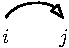
\includegraphics[scale=1.5]{figures/scoring-part/arc.pdf}
        \caption{单弧}
        \label{fig:scoring-part-arc}
    \end{subfigure}
    \begin{subfigure}[b]{0.32\textwidth}
        \centering
        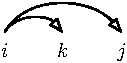
\includegraphics[scale=1.5]{figures/scoring-part/sib.pdf}
        \caption{邻接兄弟}
        \label{fig:scoring-part-sib}
    \end{subfigure}
    \begin{subfigure}[b]{0.32\textwidth}
        \centering
        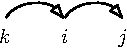
\includegraphics[scale=1.5]{figures/scoring-part/grd.pdf}
        \caption{祖父-父亲-孩子}
        \label{fig:scoring-part-grd}
    \end{subfigure}
    \caption{模型中使用的打分结构.}
    \label{fig:dep-vi-scoring-part}
\end{figure}

\subsection{推断}

\noindent\textbf{平均场变分推断}

\noindent\textbf{循环置信传播}

\subsection{训练}

\subsection{解码}

\section{实验}\label{sec:dep-vi-exp}

头选择(head selection)的结构约束要求句子中除了根结点之外的每个词有且仅有一个头.
我们定义变量$\boldsymbol{y}_j\in \{0,1,\cdots,n\}$来表示词$w_j$的头索引.
之后,我们在变量$\boldsymbol{y}= [\boldsymbol{y}_0,\boldsymbol{y}_1,\cdots,\boldsymbol{y}_n]$的基础上定义条件随机场.
具体地,对于每个变量$\boldsymbol{y}_j$,一阶的势函数(potential function)定义为
\begin{equation}
    \label{eq:1o-potential}
    \psi_u(\boldsymbol{y}_j=i)=\exp(s(i, j))
\end{equation}
而给定两个变量$\boldsymbol{y}_j$和$\boldsymbol{y}_k$,二阶的势函数定义为
\begin{equation}
    \label{eq:2o-potential}
    \psi_b(\boldsymbol{y}_j=i,\boldsymbol{y}_k=l)=\left\{
    \begin{array}{rcl}
        \exp \mathrm{s}^{sib}(i,k,j) &  & {i=l}       \\
        \exp \mathrm{s}^{grd}(i,k,j) &  & {l=j}       \\
        1                            &  & {otherwise}
    \end{array}
    \right.
\end{equation}

\section{实验}\label{sec:dep-vi-exp}

\subsection{主要结果}

\begin{table}[tb!]
  \centering
  \begin{tabular}{lcccc}
    \toprule
             & \multicolumn{2}{c}{PTB} & \multicolumn{2}{c}{CoNLL09}                 \\
             & UAS                     & LAS                         & UAS   & LAS   \\[2pt]
    \hline
    \\[-15pt]
    Baseline & 95.72                   & 93.97                       & 88.80 & 85.86 \\[3pt]
    LBP      &                         &                             &       &       \\
    MFVI     &                         &                             &       &       \\
    \bottomrule
  \end{tabular}
  \caption{Dev数据上的结果.}
  \label{table:dev-test}
\end{table}




\subsection{分析}

\noindent\textbf{局部和全局因子的影响.}

\noindent\textbf{子树和完全树的结果.}

\noindent\textbf{数据量的影响.}

\noindent\textbf{迭代次数的影响.}

\subsection{样例分析}

\subsection{速度比较}

\subsection{UD的结果}
